% =====================================================================
%  Sohrab Rana – Lebenslauf (Deutsch)
%  Compiler: pdfLaTeX  (Overleaf: Menu -> Compiler -> pdfLaTeX)
%  Layout:   eine A4-Seite, einspaltig, ATS-freundlich
%            (keine Tabellen, Icons, Spalten, Textboxen oder Grafiken)
%  Optional: Bewerbungsfoto -> \showphototrue setzen und photo.jpg
%            in denselben Ordner legen (für ATS-Uploads besser ohne Foto).
% =====================================================================
\documentclass[10pt,a4paper]{article}

% ---------- Kodierung: Text bleibt für ATS auslesbar ----------
\usepackage[T1]{fontenc}
\usepackage[utf8]{inputenc}
\input{glyphtounicode}
\pdfgentounicode=1

% ---------- Schrift & Typografie ----------
\usepackage[sfdefault,scale=0.93]{plex-sans} % IBM Plex Sans
\usepackage[ngerman]{babel}
\usepackage{microtype}
\usepackage[none]{hyphenat}                  % keine Silbentrennung: Schlüsselwörter bleiben ganz
\usepackage[a4paper,left=1.45cm,right=1.45cm,top=0.7cm,bottom=0.8cm]{geometry}
\usepackage{xcolor}
\usepackage{enumitem}
\usepackage{titlesec}
\usepackage{eso-pic}                       % header band (vector shape, no image)
\usepackage{graphicx}
\usepackage[hidelinks,unicode,pdfusetitle]{hyperref}

% ---------- Farben ----------
\definecolor{ink}{HTML}{0F1E33}      % Text und Kopfband
\definecolor{accent}{HTML}{2450B8}   % Links, Arbeitgeber, Zeiträume
\definecolor{signal}{HTML}{F2B705}   % Hervorhebung
\definecolor{muted}{HTML}{52627A}
\definecolor{rule}{HTML}{C9D2DE}
\definecolor{bandtext}{HTML}{D2DBE8}
\color{ink}

% ---------- Kopfband: farbiges Rechteck hinter dem Kopfbereich ----------
% Der Text bleibt normaler, auswählbarer Text und ist für ATS lesbar.
\newlength{\bandheight}\setlength{\bandheight}{3.4cm}
\AddToShipoutPictureBG*{\AtPageUpperLeft{\color{ink}\rule[-\bandheight]{\paperwidth}{\bandheight}}}

% ---------- Foto (optional) ----------
\newif\ifshowphoto
\showphotofalse            % \showphototrue = Foto oben rechts (Datei: photo.jpg)

% ---------- Persönliche Angaben ----------
\newcommand{\cvname}{Sohrab Rana}
\newcommand{\cvheadline}{Junior Business Intelligence Analyst | Datenanalyst | Power BI Developer}
\newcommand{\cvlocation}{Duisburg}
% Telefon: beide Zeilen leer lassen ({}), um die Nummer im Kopf auszublenden.
\def\cvphone{+49 179 446 8668}
\def\cvphonelink{+491794468668}
\newcommand{\cvemail}{sohrabrana44@gmail.com}
\newcommand{\cvlinkedin}{linkedin.com/in/sohrab-rana}
\newcommand{\cvgithub}{github.com/Sohrabrana}
\newcommand{\cvportfolio}{sohrabrana.github.io}

\hypersetup{
  pdftitle={Lebenslauf Sohrab Rana - Business Intelligence Analyst, Datenanalyst, Power BI Developer},
  pdfauthor={Sohrab Rana},
  pdfsubject={Lebenslauf},
  pdfkeywords={Business Intelligence Analyst, Datenanalyst, Data Analyst, Power BI Developer, Business Analyst, Supply Chain Analyst, Power BI, DAX, Power Query, SQL, SAP ERP, KPI-Reporting, Prozessoptimierung, Power Automate},
  pdflang={de-DE}
}

% ---------- Layout-Helfer ----------
\pagestyle{empty}
\setlength{\parindent}{0pt}
\setlength{\parskip}{0pt}
\raggedright
\linespread{1.0}

\titleformat{\section}
  {\color{ink}\large\bfseries}
  {}{0pt}{{\color{signal}\rule[-0.22ex]{0.3em}{1.05em}}\hspace{0.45em}}
  [\vspace{-0.55em}{\color{rule}\rule{\linewidth}{0.6pt}}]
\titlespacing*{\section}{0pt}{0.5em}{0.26em}

\setlist[itemize]{leftmargin=1.05em,label={\color{accent}\textbullet},
  itemsep=0.5pt,parsep=0pt,topsep=1.2pt,partopsep=0pt}

% \role{Position}{Zeitraum}{Arbeitgeber}{Ort}
\newcommand{\role}[4]{%
  \vspace{0.22em}%
  {\bfseries #1}\par
  {\color{accent}\bfseries #2} | {\color{accent}#3} | {\color{muted}#4}\par}

% \entry{Titel}{Zeitraum}  – für Projekte und Ausbildung
\newcommand{\entry}[2]{%
  \vspace{0.22em}%
  {\bfseries #1} | {\color{muted}#2}\par}

\newcommand{\skill}[2]{{\bfseries #1:} #2\par\vspace{0.12em}}

% =====================================================================
\begin{document}

% ---------- Kopfzeile ----------
\ifshowphoto\begin{minipage}[t]{0.86\linewidth}\fi
{\color{white}\fontsize{27}{29}\fontseries{bc}\selectfont \cvname\par}
\vspace{0.2em}
{\large\color{signal}\fontseries{sbc}\selectfont \cvheadline\par}
\vspace{0.35em}
{\small\color{bandtext}
\cvlocation{} | \ifx\cvphone\empty\else\href{tel:\cvphonelink}{\color{white}\cvphone} | \fi\href{mailto:\cvemail}{\color{white}\cvemail} | \href{https://www.\cvlinkedin}{\color{white}\cvlinkedin} | \href{https://\cvgithub}{\color{white}\cvgithub}\par
\vspace{0.12em}
Portfolio: \href{https://\cvportfolio}{\color{white}\cvportfolio} | Ab sofort verfügbar in Vollzeit | Deutschlandweit umzugsbereit\par}
\ifshowphoto\end{minipage}\hfill
\begin{minipage}[t]{0.1\linewidth}\vspace{0pt}\raggedleft
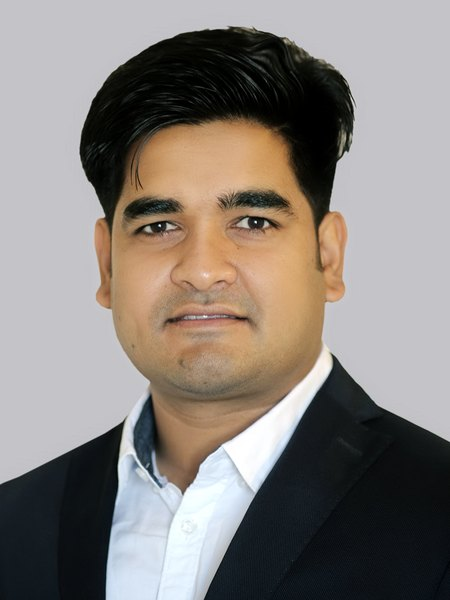
\includegraphics[width=\linewidth]{photo.jpg}
\end{minipage}\par\fi
\vspace{0.62cm}

% ---------- Profil ----------
\section{Profil}
Business Intelligence Analyst und Datenanalyst mit 1,5 Jahren Praxiserfahrung bei Uniper und Continental (Werkstudent, Praktikum). Schwerpunkte: Power-BI-Dashboards, Datenmodellierung und KPI-Reporting mit SAP-, SQL- und Excel-Daten sowie Prozessautomatisierung. B.Sc. Mobility and Logistics; M.Sc. Operations Research and Business Analytics laufend.\par
\vspace{0.2em}
{\bfseries Kernkompetenzen:} {\color{accent}\bfseries Power BI | DAX | Power Query | SQL | SAP ERP | Datenmodellierung | KPI-Reporting}\par

% ---------- Berufserfahrung ----------
\section{Berufserfahrung}

\role{Werkstudent – Operational Excellence / Transformation \& Excellence}{04/2025 – 04/2026}
     {Uniper Global Commodities SE}{Düsseldorf (hybrid)}
\begin{itemize}
  \item Entwicklung und Veröffentlichung von \textbf{5 Power-BI-Dashboards} für das Management- und operative KPI-Reporting
  \item Datenaufbereitung und Datenmodellierung (Microsoft 365, SharePoint, Microsoft Forms) mit Power Query, DAX und Excel; Betreuung der automatisierten Datenaktualisierung
  \item Umsetzung eines KI-Agenten mit Microsoft Copilot Studio für ein SharePoint-basiertes Wissensmanagement-Portal
  \item Automatisierung von Arbeitsabläufen mit Power Automate und Power Apps; Prozessanalyse und Prozessoptimierung
  \item Begleitung der Einführung von Microsoft 365 Copilot mit Praxisbeispielen und \textbf{4 Praxisschulungen} zu Copilot-Agenten; Vorstellung der Dashboard-Updates in monatlichen Teammeetings
\end{itemize}

\role{Praktikant – Microsoft Power BI und Effizienzmaßnahmen}{08/2024 – 01/2025}
     {Continental – ADC Automotive Distance Control Systems GmbH}{Lindau (Bodensee)}
\begin{itemize}
  \item Entwicklung von Power-BI-Dashboards und Datenmodellen in \textbf{8 Projekten} der Application Engineering Excellence, u.\,a. Europa-Wochenreports, Prototypenkosten, EBOM (Engineering-Stückliste), Umfrageauswertung
  \item Extraktion, Transformation und Validierung von Daten aus SAP ERP, SQL-Datenbanken, SharePoint, JIRA und Excel/CSV mit Power Query und DAX; Automatisierung der Datenaufbereitung mit Excel-VBA, Makros und KNIME
  \item Maßgeschneiderte Dashboards für Stakeholder in Europa, Nordamerika, China, Japan, Korea und Rumänien
  \item Freiwillige Verlängerung (remote, 01/2025 – 04/2025): Weiterentwicklung der Dashboards, Datenvalidierung
\end{itemize}

\vspace{0.22em}%
{\bfseries Verkaufsberater (Studentenjob neben dem Studium)}, {\color{accent}H\&M über Studitemps GmbH}, Köln | {\color{muted}02/2021 – 08/2024}\par

% ---------- Projekte ----------
\section{Projekte}

\entry{Bachelorarbeit: Einführung von Microsoft 365 Copilot bei Uniper (Note 2,0)}{01/2026 – 05/2026}
\begin{itemize}
  \item Analyse von Microsoft-365-Nutzungsdaten, einer Mitarbeiterbefragung und Experteninterviews auf Basis des UTAUT-Modells; Power-BI-Dashboard und \textbf{7 Handlungsempfehlungen}
\end{itemize}

\entry{SQL- und Power-BI-Portfolioprojekte (synthetische Daten) – \href{https://github.com/Sohrabrana}{github.com/Sohrabrana}}{2026}
\begin{itemize}
  \item \textbf{Lieferperformance-Analyse:} MySQL-Datenmodell mit Datenqualitätsprüfungen; CTEs, Fensterfunktionen und P90-Lieferzeiten für Versanddienstleister- und Lager-Scorecards; Sternschema mit \textbf{20 DAX-Measures}
  \item \textbf{Bestands- und Einkaufsanalyse:} 16 Fachfragen mit JOINs, Aggregationen und Unterabfragen; Lieferanten-Scorecard
\end{itemize}

% ---------- Kenntnisse ----------
\section{IT-Kenntnisse}
\skill{BI \& Reporting}{Power BI (Desktop \& Service), DAX, Power Query, Datenmodellierung (Sternschema), Datenvisualisierung}
\skill{Daten \& Systeme}{SQL (MySQL), Python (gute Kenntnisse), Excel (VBA/Makros), SAP ERP, SharePoint, JIRA, KNIME}
\skill{Automatisierung \& KI}{Power Automate, Power Apps, Microsoft Copilot Studio, Microsoft 365 Copilot}
\skill{Methoden}{KPI-Reporting, Datenvalidierung, Prozessanalyse, Prozessoptimierung, Lean Six Sigma, Schulungen}

% ---------- Ausbildung ----------
\section{Ausbildung}
\entry{M.Sc. Operations Research and Business Analytics – Otto-von-Guericke-Universität Magdeburg}{seit 10/2026}
\entry{B.Sc. Mobility and Logistics – Hochschule Rhein-Waal}{10/2021 – 05/2026}
{\small Schwerpunkte: Datenmanagement, Statistik, Wirtschaftsinformatik (SAP), Lineare Optimierung, Supply Chain Management\par}

% ---------- Zertifikate ----------
\section{Zertifikate und Weiterbildungen}
{\small
Mastering BI with DAX, Power BI and Excel, LinkedIn Learning (2026) | Lean Six Sigma Yellow Belt, Uniper (2026) | McKinsey Forward Program (2026) | Copilot Studio Masterclass, Udemy (2025) | Power BI, 365 Data Science (2024) | SAP University Alliances Zertifikat (2022)\par}

% ---------- Sprachen ----------
\section{Sprachkenntnisse}
Bengalisch: Muttersprache | Englisch: C1 (verhandlungssicher) | Deutsch: B1 (telc-Zertifikat 2026, B2 in Vorbereitung)

\end{document}
